\section{Funzioni}

\begin{center}
	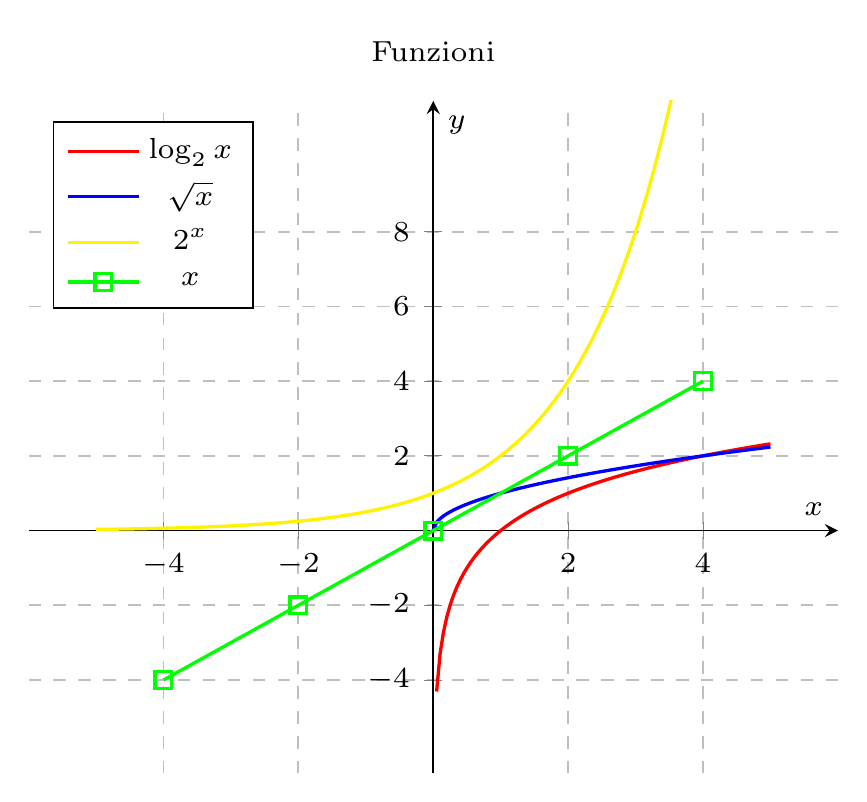
\begin{tikzpicture}[scale=1.5]
		\begin{axis}[
				title={Funzioni},
				font=\scriptsize,
				axis lines = center,
				xlabel = $x$,
				ylabel = $y$,
				xtick = {-4, -2, 2, 4},
				ytick = {-4, -2, 2, 4, 6, 8},
				ymin = -5, ymax = 10,
				xmin = -5, xmax = 5,
				grid = both,
				grid style = dashed,
				legend pos = north west,
				enlargelimits
			]

			\addplot [
				domain=0:5,
				samples=100,
				thick,
				color=red
			]
			{log2(x)};
			\addlegendentry{$\log_2{x}$};

			\addplot [
				domain=0:5,
				samples=100,
				thick,
				color=blue
			]
			{sqrt(x)};
			\addlegendentry{$\sqrt{x}$};

			\addplot [
				domain=-5:5,
				samples=100,
				thick,
				color=yellow,
			]
			{2^x};
			\addlegendentry{$2^x$};

			\addplot [
				domain=-5:5,
				samples=100,
				thick,
				color=green,
				mark=square
			]
			coordinates {(-4, -4) (-2, -2) (0, 0) (2, 2) (4, 4)};
			\addlegendentry{$x$};

		\end{axis}
	\end{tikzpicture}
\end{center}

\begin{center}
	\begin{tikzpicture}
		\begin{axis}[
				% standard,
				xtick={-2, -1, 1, 2},
				xticklabels={-2, -1, 1, 2},
				ytick={-2, -1, 1, 2},
				yticklabels={-2, -1, 1, 2},
				samples=1000,
				xmin=-2, xmax=2, ymin=-2, ymax=2
			]
			\node[anchor=center, label=south west: $O$] at (axis cs: 0, 0){};

			\addplot[name path=F, domain={-3:3}, thick, blue] {x^3 + x^2 - x - 0.5};

			\path[name path=xAxis] (axis cs:-1.45, 0) -- (axis cs:0.85, 0);
			\addplot[fill=blue, fill opacity=0.2] fill between [of=F and xAxis, soft clip={domain=-1.45:0.85}];
		\end{axis}
	\end{tikzpicture}
\end{center}